\section{Przypadek Testowy 6 - Tabu Search - zależność PRD od maksymalnej liczby iteracji bez poprawy}
  \subsection{Cel:}
    W tej części zostaną ze sobą porównane PRD rozwiązania algorytmu Tabu Search w zależności od maksymalnej liczby iteracji bez poprawy.
    \subsection{Założenia:}
    Do badania tego przypadku zostały wykorzystane instancje grafów z paczki tsp. Dodatkowo maksymalna długość listy tabu równa 50, maksymalna liczba iteracji równa 200 oraz liczba sąsiadów równa 10\% wszystkich węzłów w grafie (zaokrąglona w dół). Ponad to dla każdej instancji ilość iteracji została ograniczona w zakresie od 10 do 100 z iteracjią co 10;
  \subsection{Wyniki: }
    Ze względu na czytelność wszystkie wyniki są załączone w pliku \textbf{out\_test\_3.csv}.
  \subsection{Wykresy: }
    \begin{figure}[H]
      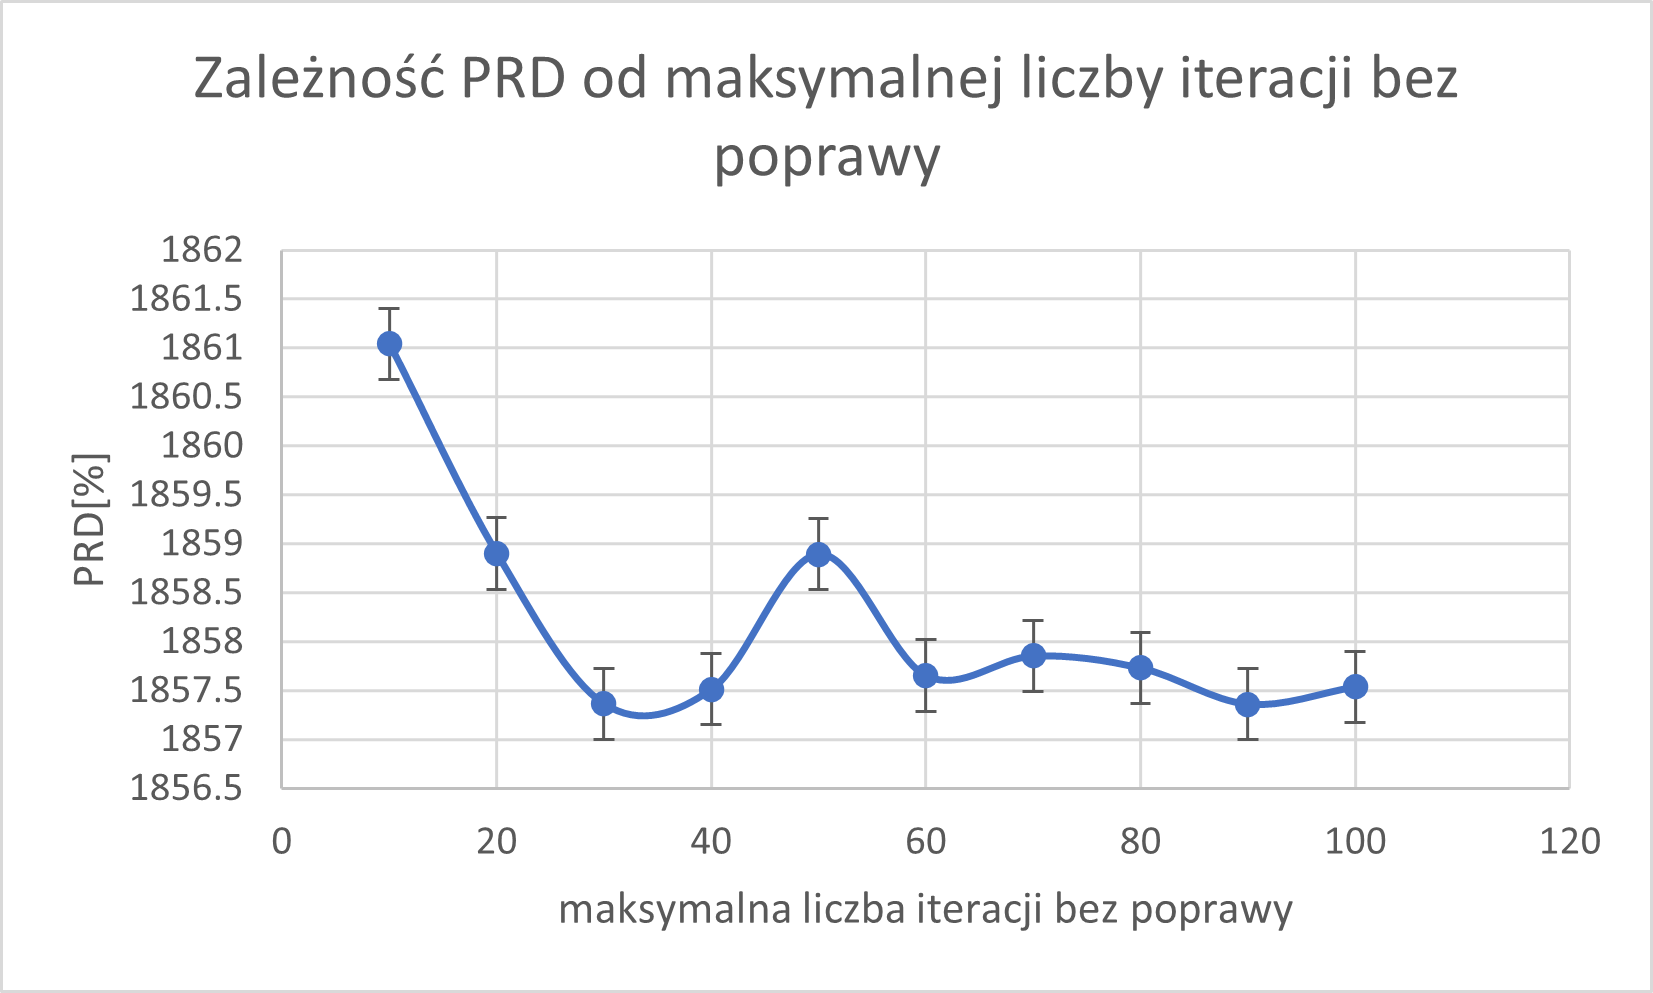
\includegraphics[scale=0.75]{chart_test3_1.png}
      \centering
      \caption{zależność PRD od maksymalnej liczby iteracji bez poprawy}
    \end{figure}
    
    Na wykresach przedstawione są średnie wartości PRD dla badanych danych.

    Odchylenie standardowe oraz błąd standardowy zostały obliczone według wzorów: \\
    Odchylenie standardowe:
    \[ \sigma = \sqrt{\frac{\sum_{n = 1}^{10}(\bar{x} - x_n)^2}{10}} \]
    Błąd standardowe:
    \[ \sigma_{\bar{x}} = \frac{\sigma}{\sqrt{10}} \]

  \subsection{Wnioski: }
    Zauważmy, że dla danych testowych poprawa jakości rozwiązania względem zwiększania maksymalnej liczby iteracji nie jest wprost rosnąca/malejąca. Jednak można zauważyć że większa większa liczba iteracji bez poprawy w zakresie \{10, 40\} wpływa na poprawe jakości rozwiązania. Przyglądając się poszczególnym przypadkom można zauważyć takie w których zmiana maksymalnej liczby iteracji bez poprawy nie zmienia jakości rozwiązania, jak i takie przypadki gdzie jakość rozwiązania stabilizuje się.

